\documentclass[
    aspectratio=169,   % アスペクト比。基本的に169(=16:9)でよい
    xcolor={           % Beamerはxcolorも自動で読み込むので、パラメータ指定
        rgb,           %   ・Hsb色指定のためにrgbを設定
        svgnames},     %   ・指定可能色名:https://www.latextemplates.com/svgnames-colors
    unicode,           % LuaLaTeXを使用する上で要指定
    12pt,              % 基準フォントサイズ
    unknownkeysallowed % 未定義のキーによるエラーを無視
]{beamer}

\usetheme{satori} % 使用beamerテーマ
%% パス指定で使用する場合(テーマファイルが同階層に無いなど)は以下
%\usepackage{themeFiles/beamerthemesatori}

%% 色相指定(コメントアウトでモノクロ)
\defineColorWithHue{30} % 0-360

%% ロゴ画像指定(ロゴ表示しない場合はコメントアウト)
\renewcommand{\logoImage}{png/SATORI.png}

%% ウォーターマーク(表示しない場合はコメントアウト)
%% \waterMark{画像}{不透明度}{サイズ(1=画面一杯)}{x座標移動}{y座標移動}{回転(反時計回り)}
\waterMark{png/SATORI2.png}{.03}{1.2}{3cm}{-.8cm}{0}

%% 和暦表示にしたい場合、以下の2行をコメントアウト解除
%\usepackage{bxwareki}
%\renewcommand{\today}{\warekitoday}

%% タイトル類
\titlePattern{A} % タイトル頁のテーマ:A-Jを指定
\title{サンプル}
%\subtitle{Hoge}
\author{SATORI}
%\institute{Fuga}
\date{\today}

\usepackage{pgfplots} % TikZによるグラフ描画

%%%%%%%%%%%%%%%%%%%%%%%%%%%%%%%%%%%%%%%%%%%%%%%%%%%%%%%%%%%%%%%%%%%%%%%%%%%%%%%%%%%%%%%%%%%%%%%%%%%%
\begin{document}

\begin{frame}[plain,b]
  \titlepage
\end{frame}


%%%%%%%%%%%%%%%%%%%%%%%%%%%%%%%%%%%%%%%%
\section{文字スライド}

%%%%%%%%%%%%%%%%%%%%
\begin{frame}[fragile]{文字表示と各種装飾}
  あの\textcolor{red}{イーハトーヴォ}の\underline{すきとほつた風}、夏でも底に冷たさをもつ\textcolor{blue}{\underline{\textcolor{modernDarkBlue}{靑いそら}}}、
  \textserif{\textlt{うつくしい森}で\CID{13844}られた\textbf{モリーオ市}、郊外の}ぎらぎらひかる{\large 草の波}。\par
  またそのなかでいつしよになつた、たくさんのひとたち、\textbf{ファゼーロ}と\texteb{ロザーロ}、羊\CID{08700}のミーロや、
  たくさんの顏の赤いこどもたち、地主のテーモ、山猫\CID{13976}士の{\scriptsize ボーカント・デステゥパーゴ}、
  などいまこの暗い\ruby{巨}{おほ}きな\fbox{石の建物}のなかで考へてみますと、みな、むかし風のなつかしい靑い\ruby{幻燈}{げん|とう}のやうに思はれます。

  ※各装飾の指定方法はsample.texファイルをご覧ください。
\end{frame}

%%%%%%%%%%%%%%%%%%%%%%%%%%%%%%%%%%%%%%%%
\section{コード表示}

%%%%%%%%%%%%%%%%%%%%
\begin{frame}[fragile]{ソースコード}
  \begin{block}{ソースコードサンプル}
    \begin{lstlisting}
      public class Hello {
          public static void main(String[] args) {
              System.out.println("Hello, World."); // コンソール出力
          }
      }
    \end{lstlisting}
  \end{block}

  \lstinline{String hoge = null;}⬅インライン表示も可能。

  beamerでソースコード表示する場合、フレームにfragile指定が必要。\\
  ➡例:\lstinline|\begin{frame}[fragile]{Hoge}|

  注意点:fragileフレームは\lstinline|\begin{frame}|から\lstinline|\end{frame}|の間が\textcolor{red}{2行以上空いてないとエラーになる}模様(空行でも可)。
\end{frame}

%%%%%%%%%%%%%%%%%%%%%%%%%%%%%%%%%%%%%%%%
\section{いろんなブロック}

%%%%%%%%%%%%%%%%%%%%
\begin{frame}[fragile]{ブロック3種}
  \begin{block}{通常ブロック}
    これは通常ブロックです。
  \end{block}

  \begin{alertblock}{警告ブロック}
    これは警告ブロックです。
  \end{alertblock}

  \begin{exampleblock}{例示ブロック}
    これは例示ブロックです。
  \end{exampleblock}
  用途は自由。警告ブロックだからといって警告専用ではない。
\end{frame}

%%%%%%%%%%%%%%%%%%%%%%%%%%%%%%%%%%%%%%%%
\section{画像}

%%%%%%%%%%%%%%%%%%%%
\begin{frame}[fragile]{画像表示}
  ↓画像を挿入可能↓\\
  \centering
  \includegraphics[height=5cm]{\logoImage}\\
  ↑画像を挿入可能↑
\end{frame}

%%%%%%%%%%%%%%%%%%%%%%%%%%%%%%%%%%%%%%%%
\section{カラム(左右分割)}

%%%%%%%%%%%%%%%%%%%%
\begin{frame}[fragile]{左右分割}
  \begin{columns}[c, onlytextwidth]
    \begin{column}{.4\textwidth}
      \centering
      \includegraphics[width=5cm]{\logoImage}
      \begin{block}{テスト}
        左右分割テスト
      \end{block}
    \end{column}
    \begin{column}{.55\textwidth}
      左右分割することで、図やソースコードを補足説明するスライドなどが簡単に実現できる。\par
      ちなみに3分割以上も可能。
    \end{column}
  \end{columns}
\end{frame}


%%%%%%%%%%%%%%%%%%%%%%%%%%%%%%%%%%%%%%%%
\section{箇条書き}

%%%%%%%%%%%%%%%%%%%%
\begin{frame}[fragile]{箇条書き}
  \begin{itemize}
    \item 箇条書きができる
    \pause
    \item 「\verb|\pause|」を書いた箇所で
    \pause
    \item 一時停止させることも可能
  \end{itemize}
  \pause
  \begin{enumerate}
    \item 数字付きの箇条書きもできる
    \item 入れ子構造も可能
    \begin{enumerate}
      \item 入れ子
      \item 入れ子
    \end{enumerate}
    \item 通常/数字付きを混ぜることも可能
    \begin{itemize}
      \item 入れ子
      \begin{itemize}
        \item 更に入れ子
      \end{itemize}
    \end{itemize}
  \end{enumerate}
  \pause
  一時停止コマンド「\verb|\pause|」は
  \pause
  箇条書き外でも使用可能。
\end{frame}


%%%%%%%%%%%%%%%%%%%%%%%%%%%%%%%%%%%%%%%%
\section{引用}

%%%%%%%%%%%%%%%%%%%%
\begin{frame}[fragile]{引用}
  「\verb|\quoteBox{引用文}{出典}|」で引用文ボックスを作成可能。
  \quoteBox{
    あのイーハトーヴォのすきとほつた風、夏でも底に冷たさをもつ靑いそら、うつくしい森で\CID{13844}られたモリーオ市、郊外のぎらぎらひかる草の波。
  }{宮澤賢治『ポラーノの廣場』}
  背景色を変更したい場合、プリアンブルで\verb|quotationBg|を設定すること。\\
  \hugeCenterWithArrow{red}{とっても簡単、引用ボックス}
\end{frame}

%%%%%%%%%%%%%%%%%%%%%%%%%%%%%%%%%%%%%%%%
\section{このテーマについての補足}

%%%%%%%%%%%%%%%%%%%%
\begin{frame}[fragile]{色相カラーテーマ}
  それぞれの色相には固有の明度があり、明度・彩度が同じであっても色によって或いは明るく、或いは暗くなる(黄色は特に明るく、青は特に暗い)。\\
  このSatoriテーマでは、プリアンブルに\lstinline|\defineColorWithHue{数字}|と書けば指定した色相に応じて自動でそこそこ良い感じの色になる。\\
  \vspace{10pt}
  \begin{columns}[c, onlytextwidth]
    \begin{column}{.48\textwidth}
      \centering
      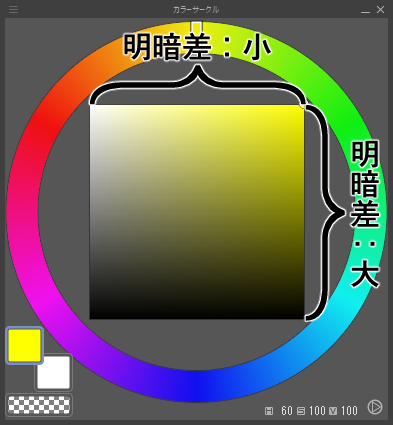
\includegraphics[width=4cm]{png/yellow.png}
    \end{column}
    \begin{column}{.48\textwidth}
      \centering
      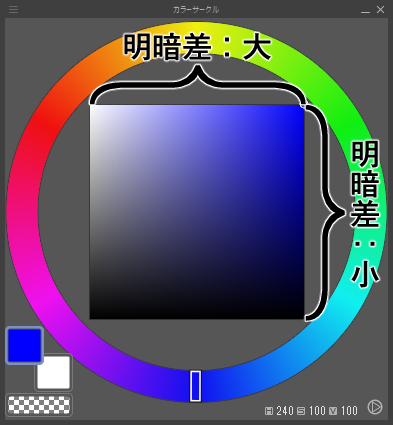
\includegraphics[width=4cm]{png/blue.png}
    \end{column}
  \end{columns}
\end{frame}

%%%%%%%%%%%%%%%%%%%%
\begin{frame}[fragile]{明度・彩度Maxの各色相}
  \definecolor{c000}{Hsb}{0, 1, 1}
  \definecolor{c010}{Hsb}{10, 1, 1}
  \definecolor{c020}{Hsb}{20, 1, 1}
  \definecolor{c030}{Hsb}{30, 1, 1}
  \definecolor{c040}{Hsb}{40, 1, 1}
  \definecolor{c050}{Hsb}{50, 1, 1}
  \definecolor{c060}{Hsb}{60, 1, 1}
  \definecolor{c070}{Hsb}{70, 1, 1}
  \definecolor{c080}{Hsb}{80, 1, 1}
  \definecolor{c090}{Hsb}{90, 1, 1}
  \definecolor{c100}{Hsb}{100, 1, 1}
  \definecolor{c110}{Hsb}{110, 1, 1}
  \definecolor{c120}{Hsb}{120, 1, 1}
  \definecolor{c130}{Hsb}{130, 1, 1}
  \definecolor{c140}{Hsb}{140, 1, 1}
  \definecolor{c150}{Hsb}{150, 1, 1}
  \definecolor{c160}{Hsb}{160, 1, 1}
  \definecolor{c170}{Hsb}{170, 1, 1}
  \definecolor{c180}{Hsb}{180, 1, 1}
  \definecolor{c190}{Hsb}{190, 1, 1}
  \definecolor{c200}{Hsb}{200, 1, 1}
  \definecolor{c210}{Hsb}{210, 1, 1}
  \definecolor{c220}{Hsb}{220, 1, 1}
  \definecolor{c230}{Hsb}{230, 1, 1}
  \definecolor{c240}{Hsb}{240, 1, 1}
  \definecolor{c250}{Hsb}{250, 1, 1}
  \definecolor{c260}{Hsb}{260, 1, 1}
  \definecolor{c270}{Hsb}{270, 1, 1}
  \definecolor{c280}{Hsb}{280, 1, 1}
  \definecolor{c290}{Hsb}{290, 1, 1}
  \definecolor{c300}{Hsb}{300, 1, 1}
  \definecolor{c310}{Hsb}{310, 1, 1}
  \definecolor{c320}{Hsb}{320, 1, 1}
  \definecolor{c330}{Hsb}{330, 1, 1}
  \definecolor{c340}{Hsb}{340, 1, 1}
  \definecolor{c350}{Hsb}{350, 1, 1}
  \definecolor{c360}{Hsb}{360, 1, 1}
  \LARGE
  \begin{centering}
      \textcolor{c000}{\ruby{■}{0}}
      \textcolor{c010}{\ruby{■}{10}}
      \textcolor{c020}{\ruby{■}{20}}
      \textcolor{c030}{\ruby{■}{30}}
      \textcolor{c040}{\ruby{■}{40}}
      \textcolor{c050}{\ruby{■}{50}}
      \textcolor{c060}{\ruby{■}{60}}
      \textcolor{c070}{\ruby{■}{70}}
      \textcolor{c080}{\ruby{■}{80}}
      \textcolor{c090}{\ruby{■}{90}}
      \textcolor{c100}{\ruby{■}{100}}
      \textcolor{c110}{\ruby{■}{110}}
      \textcolor{c120}{\ruby{■}{120}}\\
      \textcolor{c350}{\ruby{■}{350}}\hspace{14.08\zw}\textcolor{c130}{\ruby{■}{130}}\\
      \textcolor{c340}{\ruby{■}{340}}\hspace{14.08\zw}\textcolor{c140}{\ruby{■}{140}}\\
      \textcolor{c330}{\ruby{■}{330}}\hspace{14.08\zw}\textcolor{c150}{\ruby{■}{150}}\\
      \textcolor{c320}{\ruby{■}{320}}\hspace{14.08\zw}\textcolor{c160}{\ruby{■}{160}}\\
      \textcolor{c310}{\ruby{■}{310}}\hspace{14.08\zw}\textcolor{c170}{\ruby{■}{170}}\\
      \textcolor{c300}{\ruby{■}{300}}
      \textcolor{c290}{\ruby{■}{290}}
      \textcolor{c280}{\ruby{■}{280}}
      \textcolor{c270}{\ruby{■}{270}}
      \textcolor{c260}{\ruby{■}{260}}
      \textcolor{c250}{\ruby{■}{250}}
      \textcolor{c240}{\ruby{■}{240}}
      \textcolor{c230}{\ruby{■}{230}}
      \textcolor{c220}{\ruby{■}{220}}
      \textcolor{c210}{\ruby{■}{210}}
      \textcolor{c200}{\ruby{■}{200}}
      \textcolor{c190}{\ruby{■}{190}}
      \textcolor{c180}{\ruby{■}{180}}\\
  \end{centering}
\end{frame}

%%%%%%%%%%%%%%%%%%%%
\begin{frame}[fragile]{クリスタでグレスケ化した際の明度}
    \begin{tikzpicture}
        \begin{axis}[
            xlabel=グレスケ化前の色相,
            ylabel=明度,
            xmin=0, xmax=360,
            ymin=0, ymax=100,
            xtick={0,30,60,90,120,150,180,210,240,270,300,330,360},
            xtick distance=30,
            ytick distance=10,
            width=\textwidth,
            height=.9\textheight
        ]
        \addplot[smooth,mark=*,blue] plot coordinates {
            (  0, 30)
            ( 10, 39)
            ( 20, 49)
            ( 30, 59)
            ( 40, 69)
            ( 50, 78)
            ( 60, 88)
            ( 70, 83)
            ( 80, 78)
            ( 90, 73)
            (100, 68)
            (110, 64)
            (120, 58)
            (130, 60)
            (140, 62)
            (150, 64)
            (160, 66)
            (170, 68)
            (180, 70)
            (190, 60)
            (200, 50)
            (210, 40)
            (220, 31)
            (230, 21)
            (240, 11)
            (250, 16)
            (260, 21)
            (270, 26)
            (280, 31)
            (290, 36)
            (300, 41)
            (310, 39)
            (320, 37)
            (330, 35)
            (340, 33)
            (350, 32)
            (360, 30)
        };
        \addplot[smooth,mark=none] plot coordinates {
            (  0, 30)
            (360, 30)
        };
        \addplot[smooth,mark=none] plot coordinates {
            (  0, 50)
            (360, 50)
        };
        \addplot[smooth,mark=none] plot coordinates {
            (  0, 70)
            (360, 70)
        };
        \end{axis}
    \end{tikzpicture}
\end{frame}

\end{document}
